\documentclass[main.tex]{subfiles} % Subfile-Class



% ============================================================================== %
%                            Subfile document                                    %
% ============================================================================== %

\begin{document}

% Template

\subsubsection{Liniensensor}

In der vorliegenden Abhandlung wird die Entwicklung und Evaluierung eines 
Liniensensors dargelegt. Das Ziel besteht in der Konzeption eines Sensors, 
der eine unkomplizierte Auswertung ermöglicht und dazu geeignet ist, das 
vorgegebene Klebeband (\textit{Tesa Gewebeband 4651}) zuverlässig von der Wettkampfbahn 
zu differenzieren. Die Entwicklung eines eigenständigen Liniensensors wird 
vorangetrieben durch das Bewusstsein, dass das Verlassen der Strecke ein 
signifikantes Risiko birgt. Die Eigenentwicklung eines Liniensensors ermöglicht 
eine hohe Flexibilität, da alle Komponenten selbst ausgewählt werden können.

% ===================================================================================
\subsubsection*{Anforderungen}

Das Klebeband soll auf einem rötlich gefliesten Untergrund 
detektiert werden. Eine besondere Herausforderung stellen 
dabei die gleichfarbigen Längs- und Querfugen der Fliesen dar. 
Dieser Untergrund ist in Abbildung~\ref{fig:Untergrund_Wettkampf} 
dargestellt.

\begin{figure}[H]
    \centering
    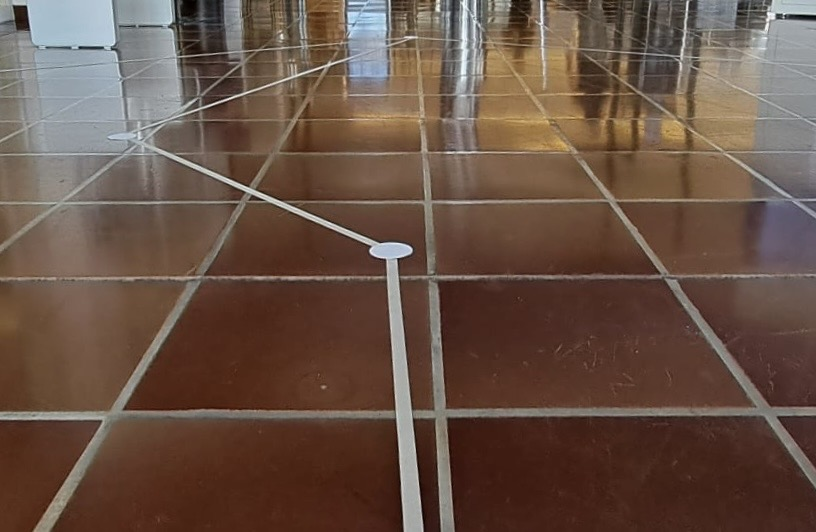
\includegraphics[width=0.75\textwidth]{fig_Strecke_Tracken/Bild_Untergrund.jpg}
    \caption{Untergrund während des Wettkampfs}~\label{fig:Untergrund_Wettkampf}
\end{figure}

% ===================================================================================

\subsubsection*{Aufbau und Auswertung}
Der Liniensensor besteht aus acht einzelnen Messzellen. Diese Anzahl wurde so 
gewählt, dass ein möglichst grosser Bereich vom Sensor abgedeckt wird, ohne 
dass zu viele Pins für die Auswertung benötigt werden. Es ist sicherzustellen, 
dass stets genau zwei Messzellen direkt über dem Klebeband ausgerichtet sind. 
Jede Messzelle besteht aus einer Leuchtdiode und einem zugehörigen 
Fototransistor. Je mehr Licht auf den Fototransistor fällt, desto höher ist 
der Strom, der durch ihn fliesst. Da der Fototransistor als Konstantstromquelle 
interpretiert werden kann, wird der Spannungspegel zwischen Widerstand und 
Transistor ausgewertet.

Ein hoher Strom durch den Fototransistor bewirkt, dass der Transistor versucht, 
mehr Strom zu liefern, als ihm der Widerstand erlaubt. Dies führt dazu, dass er 
in Sättigung gerät und das Potential stark gegen GND gezogen wird. Ist die 
Reflexion des Lichts und damit der Strom hingegen gering, lässt der 
Fototransistor weniger Strom durch, als der Widerstand zulassen würde. In 
diesem Fall bewegt sich der Spannungspegel in Richtung 3,3V. Die Spannungen 
werden anschliessend mit Analog-Digital-Wandlern (ADCs) ausgewertet. 
Abbildung~\ref{fig:Auswertung_Liniensensor1} zeigt die schematische Darstellung 
der Auswertung.
\begin{figure}[H]
    \centering
    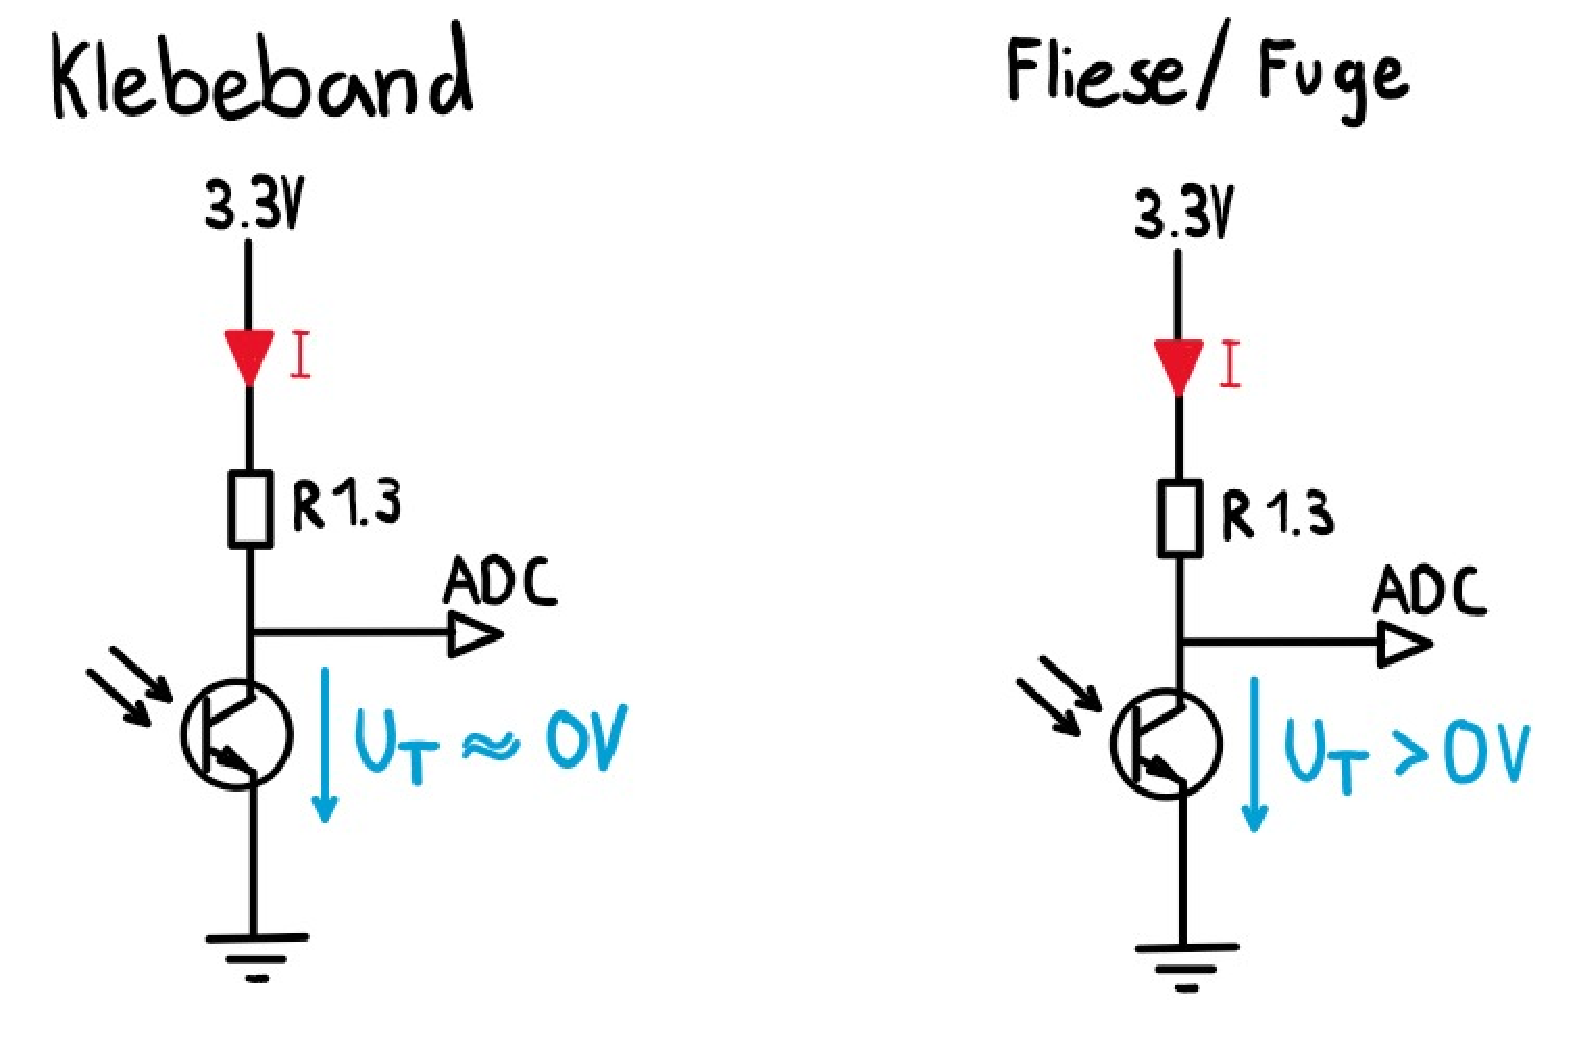
\includegraphics[width=0.5\textwidth]{fig_Strecke_Tracken/Auswertung_Liniensensor.pdf}
    \caption{Konzept der Auswertung mittels ADC}~\label{fig:Auswertung_Liniensensor1}
\end{figure}

% ===================================================================================

\subsubsection{Liniensensor als PCB}

Damit der Liniensensor möglichst praxisnah getestet werden kann, wird er als 
PCB mithilfe von KiCad entworfen. Dabei werden die oben genannten Anforderungen 
und Dimensionierungen eingehalten. In Abbildung~\ref{fig:Liniensensor_Top} 
ist die Draufsicht, und in Abbildung~\ref{fig:Liniensensor_Bottom} die 
Untersicht des PCBs dargestellt.

\begin{figure}[H]
    \centering
    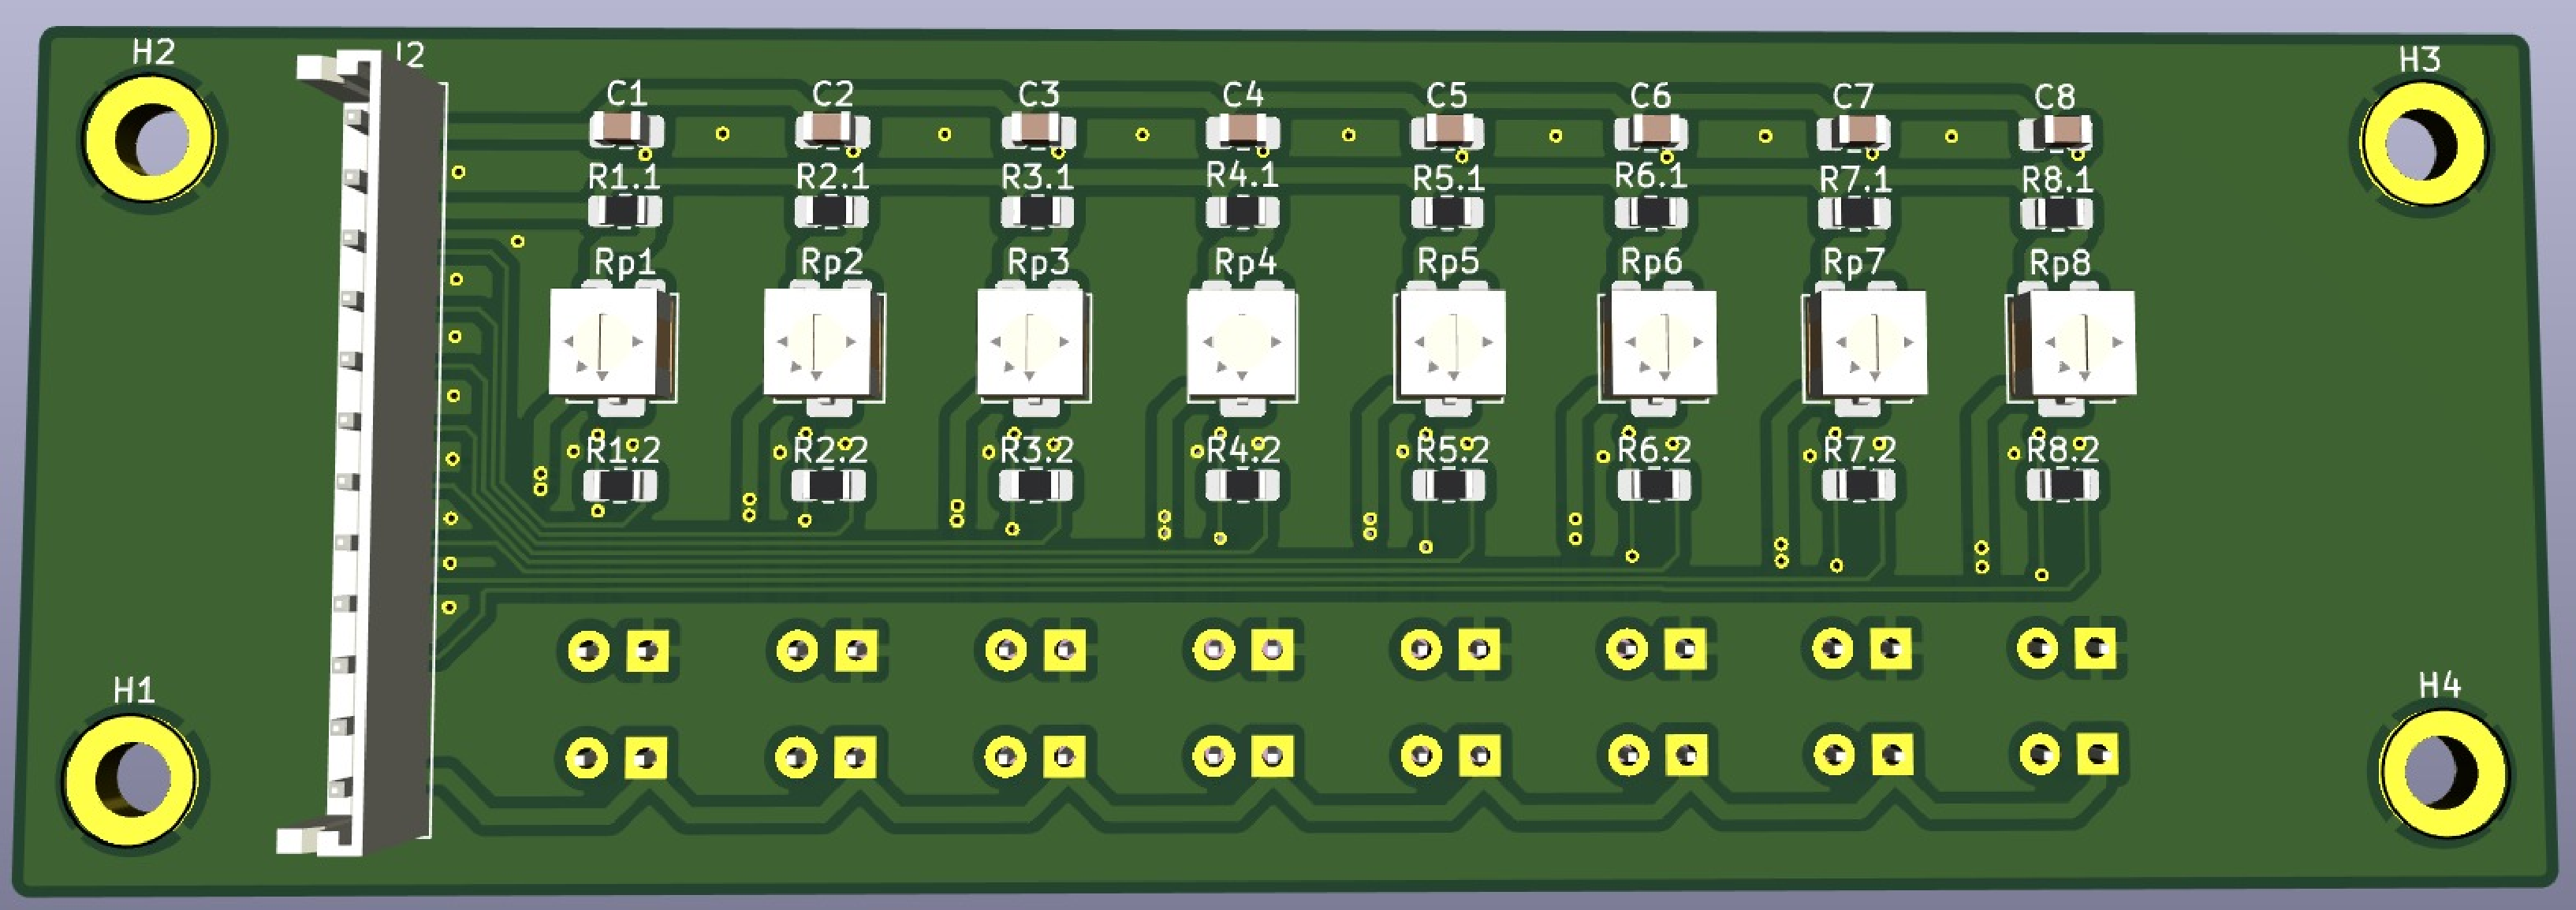
\includegraphics[width=0.75\textwidth]{fig_Strecke_Tracken/Liniensensor_Top.pdf}
    \caption{Liniensensor in Kicad von oben}~\label{fig:Liniensensor_Top}
\end{figure}

\begin{figure}[H]
    \centering
    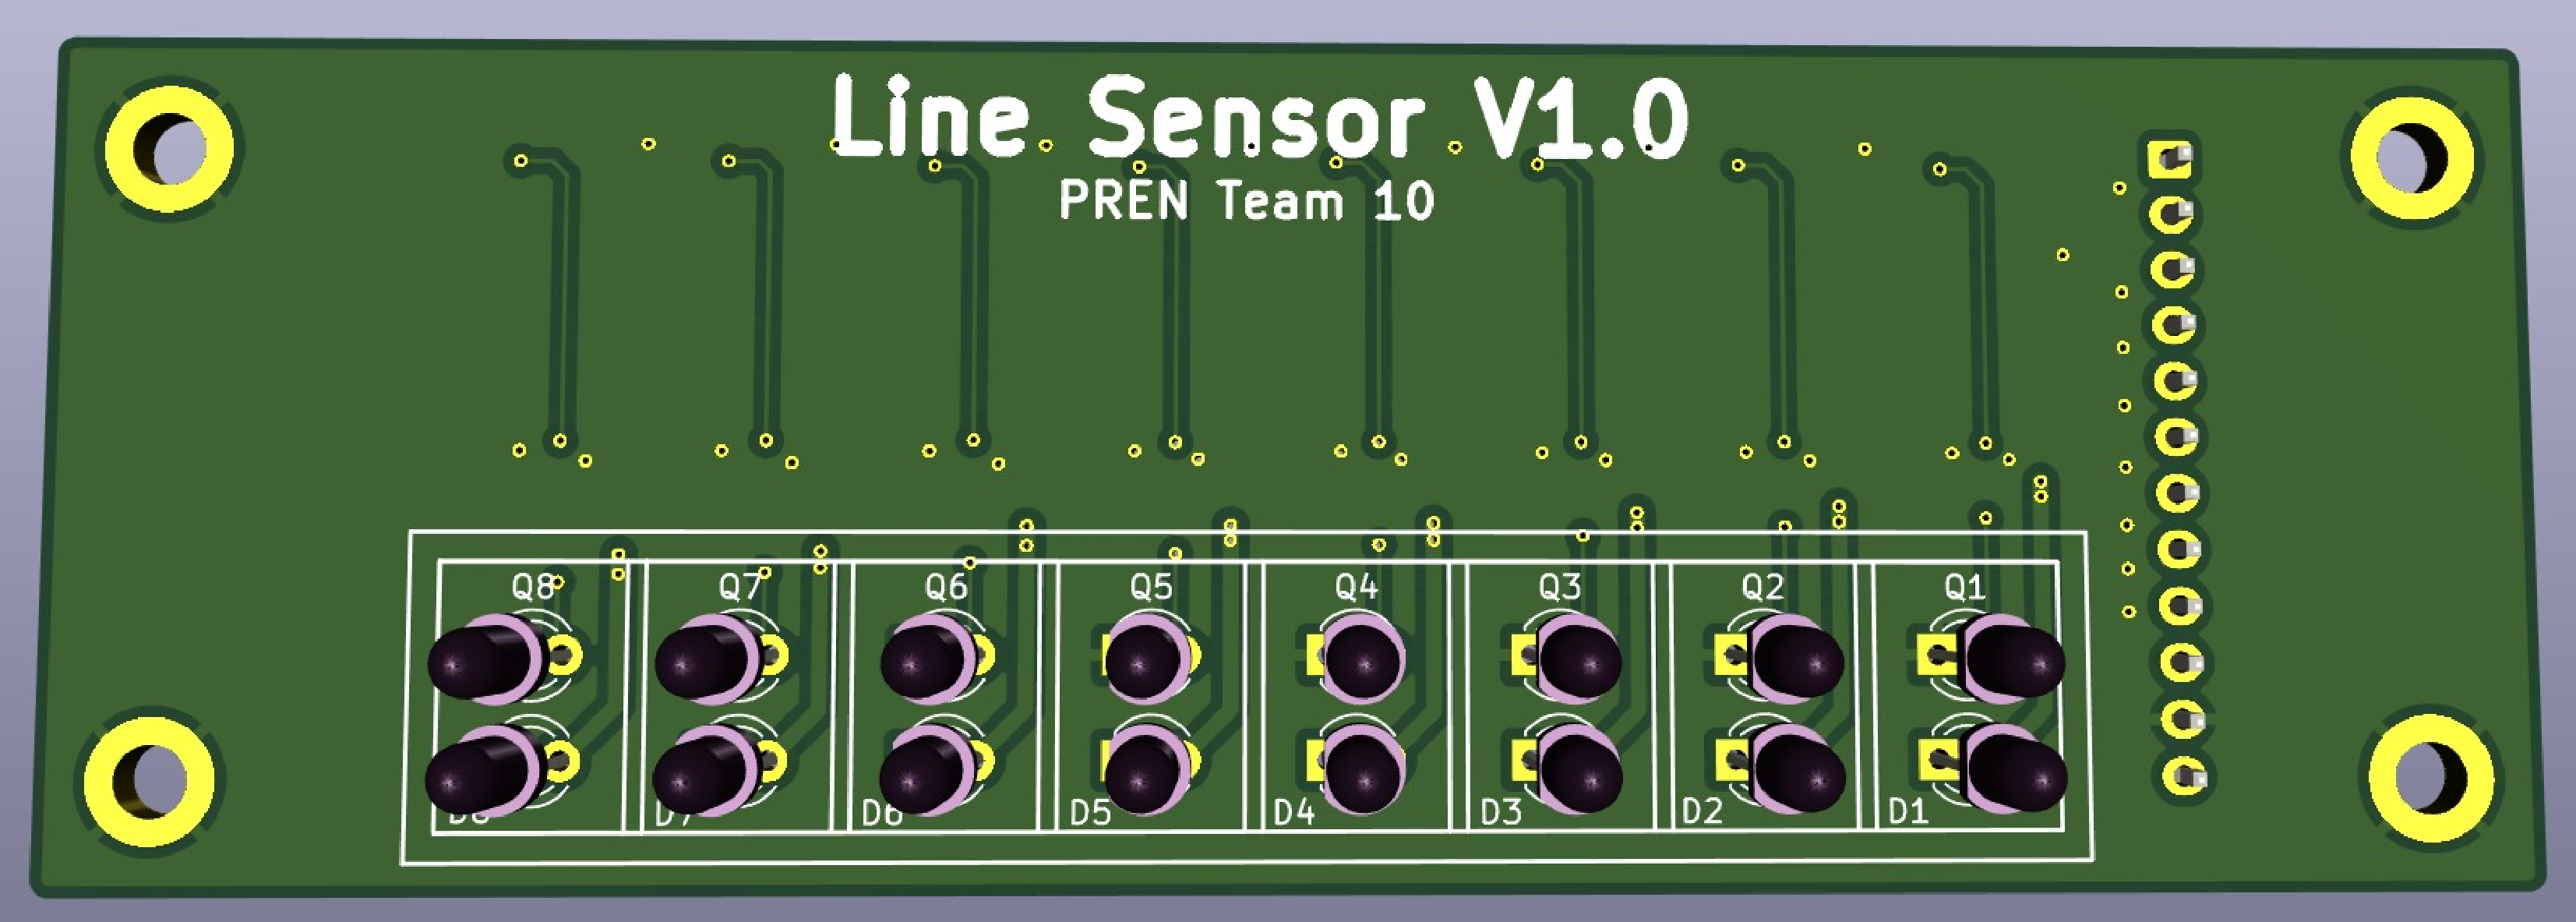
\includegraphics[width=0.75\textwidth]{fig_Strecke_Tracken/Liniensensor_Bottom.pdf}
    \caption{Liniensensor in Kicad von unten}~\label{fig:Liniensensor_Bottom}
\end{figure}

% ===================================================================================

\paragraph{Versuche}  
Im Anhang ist ein Versuch dokumentiert, der ein geeignetes Lichtspektrum für 
den Liniensensor identifiziert. Zusätzlich wurden die Ströme auf den 
unterschiedlichen Untergründen (Klebeband, Fliese und Fuge) gemessen. Mithilfe 
eines Arduino wurden alle Eingänge ausgewertet und der Liniensensor validiert. 
Die vollständigen Messungen sind im Anhang~\ref{anhang:Liniensensor} 
detailliert dargestellt.

% ===================================================================================
\paragraph{Entscheidung und Fazit}  
Durch die Messungen konnte das Konzept des Liniensensors erfolgreich überprüft 
und validiert werden. Das folgende Bild bestätigt, dass das Klebeband deutlich 
von der Fliese unterschieden werden kann. In 
Abbildung~\ref{fig:Auswertung_Strecke_Beispiel} ist die Spannungsauswertung 
mittels ADCs dargestellt. Diese Auswertung wurde mithilfe eines Arduino 
durchgeführt. Die hohen Spannungswerte repräsentieren die Fliese, während die 
tiefen Werte das Klebeband anzeigen.

\begin{figure}[H]
    \centering
    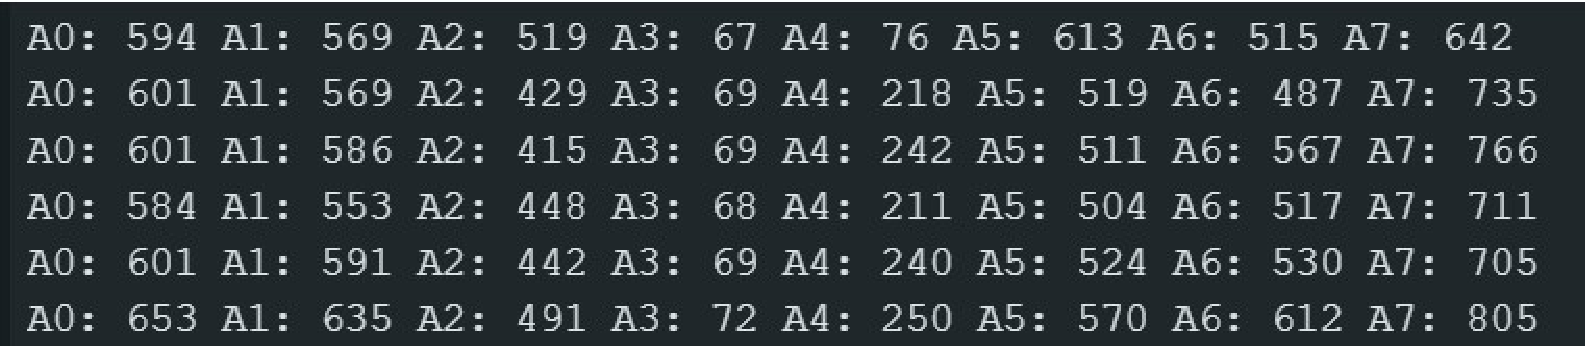
\includegraphics[width=0.75\textwidth]{fig_Strecke_Tracken/Auswertung_Strecke.pdf}
    \caption{Die tiefen Werte stellen das Klebeband dar und die hohen die Fliesen}~\label{fig:Auswertung_Strecke_Beispiel}
\end{figure}

In Abbildung~\ref{fig:Auswertung_Strecke_Beispiel} ist erkennbar, dass sich die 
Zelle A3 direkt über dem Klebeband befindet. Auch die Pins A2 und A4 liegen 
teilweise über dem Klebeband. Der gemessene Wert ist jedoch höher, da nur ein 
Teil des Klebebandes direkt darunter positioniert ist.

In der Risikobewertung wurde die Unterscheidung zwischen Klebeband und Fugen 
als potenzielles Risiko identifiziert. Der entwickelte Liniensensor ist jedoch 
in der Lage, Fugen zuverlässig von Klebebändern zu unterscheiden. Diese 
Eigenschaft ist im Anhang~\ref{anhang:Liniensensor} ausführlich dokumentiert. 
Aufgrund der klaren und reproduzierbaren Messwerte wird dieser Liniensensor 
eingesetzt.

\end{document}
